\documentclass[14pt]{extreport}
\usepackage{gost}

\begin{document}

\pagestyle{empty}

\includepdf{titulCourse.pdf}
\pagestyle{plain}

\tableofcontents

\intro

Практическая работа 2 является актуальной для первокурсников, потому что помогает им понять, какие специалисты востребованы на рынке труда и какие навыки ищут работодатели. В соответствии с этой информацией, первокурсники смогут выстроить траекторию своего обучения в высшем учебном заведении таким образом, чтобы изучать дисциплины, которые в дальнейшем помогут им устроиться на работу.

Целью данной работы является оформление отчёта в издательской системе LaTex, в соответствии с ГОСТ 7.32. Отчёт содержит 3 страницы математического текста и таблицы по 3 мечтам желаемых должностей. В каждой таблице будет представлено 5 вакансий, после таблиц будут выводы. В процессе работы будут использованы книга по математическому анализу и сайт поиска работы.

\chapter{Функция}

\section{Простейшая классификация отображений}

Когда функцию $f\colon X \to Y$ называют отображением, значение $f(x) \in Y$, которое она принимает на элементе $x \in X$, обычно называют образом элемента $x$.

Образом множества $A \subset X$ при отображении $f\colon X \to Y$ называют множество
\begin{eqnarray}
f(A) := \{y \in Y \mid \exists x \ ((x \in A)\land(y=f(x)))\}
\end{eqnarray}
тех элементов $Y$, которые являются образами элементов множества $A$.

Множество
\begin{eqnarray}
f^{-1}(B) := \{ x \in X \lor f(x) \in B\}
\end{eqnarray}
тех элементов $X$, образы которых содержатся в $B$, называют прообразом (или
полным прообразом) множества $B \subset Y$ (Рисунок~\ref{fig11}).

\begin{figure}[H]
\centerline{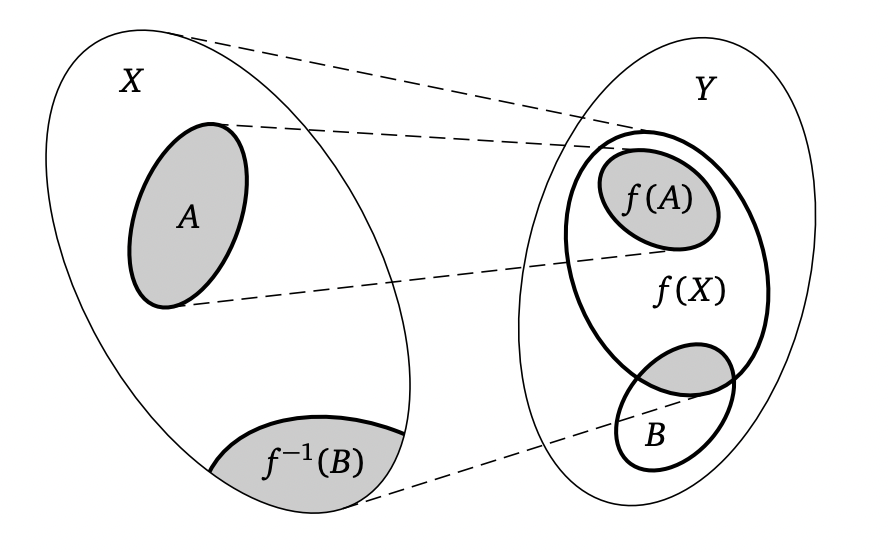
\includegraphics[width=0.5\linewidth]{extract1}}
\caption{Образы и прообразы}
\label{fig11}
\end{figure}

Про отображение $f\colon X \to Y$ говорят, что оно

сюръективно (или есть отображение $X$ на $Y$), если $f(X)=Y$;

инъективно (или есть вложение, инъекция), если для любых элементов $x_1$, $x_2$ множества $X$
\begin{eqnarray}
(f(x_1)=f(x_2)) \Rightarrow (x_1=x_2),
\end{eqnarray}
т. е. различные элементы имеют различные образы;

биективно (или взаимно однозначно), если оно сюръективно и инъективно одновременно.

Если отображение $f\colon X \to Y$ биективно, т. е. является взаимно однозначным соответствием между элементами множеств $X$ и $Y$, то естественно возникает отображение
\begin{eqnarray}
f^{-1}\colon Y \to X,
\end{eqnarray}
которое определяется следующим образом: если $f(x)=y$, то $f^{-1}(y)=x$, т. е.
элементу $y \in Y$ ставится в соответствие тот элемент $x \in X$, образом которого при отображении $f$ является $y$. В силу сюръективности $f$ такой элемент
$x \in X$ найдется, а ввиду инъективности $f$ он единственный. Таким образом,
отображение $f^{-1}$ определено корректно. Это отображение называют обратным по отношению к исходному отображению $f$.

Из построения обратного отображения видно, что $f^{-1}\colon Y \to X$ само является биективным и что обратное к нему отображение $(f^{-1})^{-1}\colon Y \to X$ совпадает с $f\colon X \to Y$.

Таким образом, свойство двух отображений быть обратными является
взаимным: если $f^{-1}$ — обратное для $f$, то, в свою очередь, $f$ — обратное
для $f^{-1}$.

Заметим, что символ $f^{-1}(B)$ прообраза множества $B \subset Y$ ассоциируется с
символом $f^{-1}$ обратной функции, однако следует иметь в виду, что прообраз
множества определен для любого отображения $f\colon X \to Y$, даже если оно не
является биективным и, следовательно, не имеет обратного.

\section{Композиция функций и взаимно обратные отображения}
Богатым источником новых функций, с одной стороны, и способом расчленения сложных функций на более простые — с другой, является операция композиции
отображений.

Если отображения $f\colon X \to Y$ и $g\colon Y \to Z$ таковы, что одно из них (в нашем
случае $g$) определено на множестве значений другого ($f$), то можно построить новое отображение
\begin{eqnarray}
g \circ f\colon X \to Z,
\end{eqnarray}
значения которого на элементах множества $X$ определяются формулой
\begin{eqnarray}
(g \circ f)(x) := g(f(x)).
\end{eqnarray}

Построенное составное отображение $g \circ f$ называют композицией отображения $f$ и отображения $g$ (в таком порядке!).

\begin{figure}[H]
\centerline{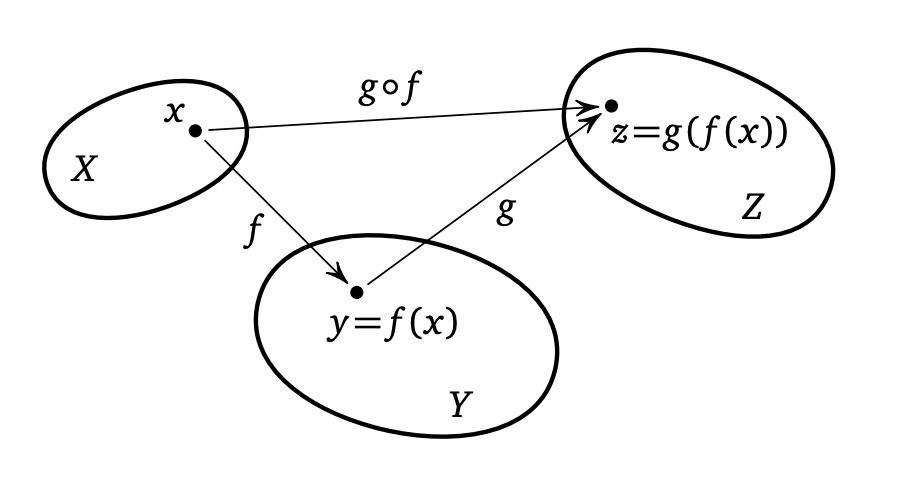
\includegraphics[width=0.5\linewidth]{extract2}}
\caption{Конструкция композиции отображений $f$ и $g$}
\label{fig12}
\end{figure}

С композицией отображений вы уже неоднократно встречались как в геометрии, рассматривая композицию движений плоскости или пространства,
так и в алгебре при исследовании «сложных» функций, полученных композицией простейших элементарных функций.

Операцию композиции иногда приходится проводить несколько раз подряд, и в этой связи полезно отметить, что она ассоциативна, т. е.
\begin{eqnarray}
h \circ (g \circ f)=(h \circ g) \circ f
\end{eqnarray}

Действительно,
\begin{eqnarray}
h \circ (g \circ f)(x)=h((g \circ f)(x))=(h \circ g)(f(x))=((h \circ g) \circ f)(x).
\end{eqnarray}

Это обстоятельство, как и в случае сложения или умножения нескольких
чисел, позволяет опускать скобки, предписывающие порядок спаривания.

Если в композиции $f_n \circ \dots \circ f_1$ все члены одинаковы и равны $f$, то ее обозначают коротко $f^n$.

Хорошо известно, например, что корень квадратный из положительного
числа $a$ можно вычислить последовательными приближениями по формуле
\begin{eqnarray}
x_{n+1}=\frac{1}{2} (x_n + \frac{a}{x_n}),
\end{eqnarray}
начиная с любого начального приближения $x_0>0$. Это не что иное, как последовательное вычисление $f^n(x_0)$, где $f(x)=\frac{1}{2}(x+\frac{a}{x})$. Такая процедура, когда вычисленное на предыдущем шаге значение функции на следующем
шаге становится ее аргументом, называется итерационным процессом. Итерационные процессы широко используются в математике.

Отметим также, что даже в том случае, когда обе композиции $g \circ f$ и $f \circ g$
определены, вообще говоря,
\begin{eqnarray}
g \circ f \ne f \circ g.
\end{eqnarray}

Действительно, возьмем, например, двухэлементное множество $\{a, b\}$ и
отображения $f \colon \{a, b\} \to a, g \colon \{a, b\} \to b$. Тогда, очевидно, $g \circ f \colon \{a, b\} \to b$, в то время как $f \circ g \colon \{a, b\} \to a$.

Отображение $f \colon X \to X$, сопоставляющее каждому элементу множества $X$
его самого, т. е. $x \xrightarrow{f} x$, будем обозначать через $e_x$ и называть тождественным отображением множества $X$.

\begin{lemma}

\begin{eqnarray}
	(g \circ f=e_x) \Rightarrow (g \text{ сюръективно})\land(f \text{ инъективно}).
\end{eqnarray}

\begin{proof} Если $f \colon X \to Y$, $g \colon Y \to X$ и $g \circ f=e_X \colon X \to X$, то
\begin{eqnarray}
X=e_X(X)=(g \circ f)(X)=g(f(X)) \subset g(Y)
\end{eqnarray}
и, значит, $g$ сюръективно.

Далее, если $x_1 \in X$ и $x_2 \in X$, то
\begin{multline}
(x_1 \ne x_2) \Rightarrow (e_X(x_1) \ne e_X(x_2)) \Rightarrow ((g \circ f)(x_1) \ne (g \circ f)(x_2)) \Rightarrow \\
\Rightarrow g(f(x_1)) \ne g(f(x_2)) \Rightarrow (f(x_1) \ne f(x_2)),
\end{multline}
следовательно, $f$ инъективно.
\end{proof}
\end{lemma}

Через операцию композиции отображений можно описать взаимно обратные отображения.
\begin{statement}
Отображения $f \colon X \to Y$, $g \colon Y \to X$ являются биективными и взаимно обратными в том и только в том случае, когда $g \circ f=e_X$ и $f \circ g=e_Y$.
\end{statement}
\begin{proof}
В силу леммы одновременное выполнение условий $g \circ f=e_X$ и $f \circ g=e_Y$ гарантирует сюръективность и инъективность, т. е. биективность каждого
из отображений $f$, $g$.

Эти же условия показывают, что $y=f(x)$ в том и только в том случае, когда $x=g(y)$.
\end{proof}
Выше мы исходили из явного построения обратного отображения. Из доказанного утверждения следует, что мы могли бы дать менее наглядное, но
зато более симметричное определение взаимно обратных отображений как
таких, которые удовлетворяют двум условиям: $g \circ f=e_X$ и $f \circ g=e_Y$.

\begin{landscape}

\chapter{Таблицы с мечтами}

\section{Мечта 1. Python разработчик}
\begin{table}[H]
\caption{Python разработчик}
\label{tab_pydev}
	\begin{tabular}{|c|p{3.3cm}|p{6cm}|p{4.7cm}|p{5.5cm}|p{3.5cm}|}
	\hline № & {Название вакансии, зарплата, ссылка} & {Требования к должности} & {Дисциплины из учебного плана} & {Преимущества} & {Недостатки} \\
	\hline 1 & {Разработчик Python,
до 300 000 руб. до вычета налогов.
Требуемый опыт работы: 3–6 лет.
Полная занятость, полный день. \url{https://clck.ru/32B6fW}} & {Уверенное знание языка и библиотек Python.
Умение работать с Git.
Опыт коммерческой разработки от 3 лет - обязателен.} & {П.4.3 Программирование;
П.4.6 Объектно-ориентированное программирование;
П.7.В1 Язык Python для анализа данных.} & {Возможность профессионального роста и влияния на технологические решения;
Официальное трудоустройство;
Стабильный и прозрачный доход.
Гибкий формат работы (офис/дом), пятидневная рабочая неделя.} & {Требуется опыт коммерческой разработки не менее 3 лет.} \\
	\hline
	\end{tabular}
\end{table}

\begin{table}[H]
	\begin{tabular}{|c|p{3.3cm}|p{6cm}|p{4.7cm}|p{5.5cm}|p{3.5cm}|}
	\multicolumn{6}{c}{Продолжение \ref{tab_pydev}} \\
	\hline № & {Название вакансии, зарплата, ссылка} & {Требования к должности} & {Дисциплины из учебного плана} & {Преимущества} & {Недостатки} \\
 	\hline 2 & {Программист Python в ООО 'Траектория', от 45 000 руб. на руки. Требуемый опыт работы: не требуется, полная занятость. \url{https://clck.ru/32B6eT}} & {Базовые знания Python3. Понимание ООП. Понимание REST API. Базовые знания SQL. Flask/Django/FastAPI. Опыт работы в Linux.} & {П.4.3 Программирование;
П.5.6 Администрирование ОС Linux;
П.4.5 Проектирование и реализация баз данных;
П.4.6 Объектно-ориентированное программирование;
П.7.В1 Язык Python для анализа данных.} & {Работа в аккредитованной IT-компании.
Свобода выбора стека технологий.
Гибкое начало дня с 8:00 до 10:00.
Молодой коллектив.} & {Испытательный срок до 3 месяцев. Минимум 1 месяц работы на условиях испытательного срока.} \\
	\hline
	\end{tabular}
\end{table}

\begin{table}[H]
	\begin{tabular}{|c|p{3.3cm}|p{6cm}|p{4.7cm}|p{5.5cm}|p{3.5cm}|}
	\multicolumn{6}{c}{Продолжение \ref{tab_pydev}} \\
	\hline № & {Название вакансии, зарплата, ссылка} & {Требования к должности} & {Дисциплины из учебного плана} & {Преимущества} & {Недостатки} \\
 	\hline 3 & {Python developer (Senior),
от 360 000 до 480 000 руб. на руки.
Требуемый опыт работы: 3–6 лет.
Полная занятость, полный день. \url{https://clck.ru/32B6fv}} & {Отличные знания Python;
Высокий уровень знаний Django; Большой опыт разработки высоконагруженных и распределенных систем;
Значительный опыт работы с SQL и NoSQL;
Опыт работы с REST API;
Опыт работы c Git.} & {П.4.3 Программирование;
П.4.5 Проектирование и реализация баз данных;
П.4.6 Объектно-ориентированное программирование;
П.7.В1 Язык Python для анализа данных.} & {Высокая оплата труда;
Интересные проекты в команде крутых специалистов;
Оплачиваемые обеды;
Лояльный график.} & {Требуется опыт от 4 лет;
Не рассматривают удаленное сотрудничество.} \\
	\hline
	\end{tabular}
\end{table}

\begin{table}[H]
	\begin{tabular}{|c|p{3.3cm}|p{6cm}|p{4.7cm}|p{5.5cm}|p{3.5cm}|}
	\multicolumn{6}{c}{Продолжение \ref{tab_pydev}} \\
	\hline № & {Название вакансии, зарплата, ссылка} & {Требования к должности} & {Дисциплины из учебного плана} & {Преимущества} & {Недостатки} \\
 	\hline 4 & {Python developer. Требуемый опыт работы: 1–3 года.
Полная занятость, полный день. \url{https://clck.ru/32B6g6}} & {Опыт коммерческой разработки от 2 лет;
Опыт разработки на Python;
Знание алгоритмов и структур данных;
Знание Английского языка (свободное чтение документации);
Хорошие коммуникативные навыки.} & {П.4.3 Программирование;
П.4.5 Проектирование и реализация баз данных;
П.4.6 Объектно-ориентированное программирование;
П.7.В1 Язык Python для анализа данных;
У.5.1 Английский язык.} & {Уютный, двухэтажный офис;
Образовательные мероприятия внутри команды, где можно обмениваться опытом;
Регулярные командные мероприятия - вместе готовим на мастер-классе или катаемся на квадроциклах.} & {Офис расположен далеко от центра СПБ.
Требуются знания в финансовой области, трейдинге для разработки рыночных стратегий.} \\
	\hline
	\end{tabular}
\end{table}

\begin{table}[H]
	\begin{tabular}{|c|p{3.3cm}|p{6cm}|p{4.7cm}|p{5.5cm}|p{3.5cm}|}
	\multicolumn{6}{c}{Продолжение \ref{tab_pydev}} \\
	\hline № & {Название вакансии, зарплата, ссылка} & {Требования к должности} & {Дисциплины из учебного плана} & {Преимущества} & {Недостатки} \\
 	\hline 5 & {Python Developer + ML
от 150 000 руб. до вычета налогов
Требуемый опыт работы: 3–6 лет
Полная занятость, полный день. \url{https://clck.ru/324t6c}} & {Опыт коммерческой разработки.
Хорошая математическая подготовка.
Навыки работы с PostgreSQL, включая опыт работы со встроенными процедурами.
Опыт работы с web, как в backend (REST API, WSS, Django), так и во frontend (второе на уровне понимания).
Знакомство с TensorFlow, Caffe, OpenVINO и общее понимание работы нейронных сетей, опыт работы с OpenCV.} & {П.4.3 Программирование;
П.4.5 Проектирование и реализация баз данных;
П.4.6 Объектно-ориентированное программирование;
П.7.В1 Язык Python для анализа данных.} & {Молодой и доброжелательный коллектив.
В офисе - кухонная зона, чай, кофе.
Расположение офиса в шаговой доступности от метро.
Возможности профессионального роста и обучения.} & {Строгие требования к кандидатам. Малоизвестная компания.} \\
	\hline
	\end{tabular}
\end{table}

Вывод: профессия python разработчика востребована на рынке труда, представлено много вакансий, которые требуют различных компетенций программирования в языке Python, требуемый опыт работы тоже варьируется.

\section{Мечта 2. Сетевой инженер}

\begin{table}[H]
\caption{Сетевой инженер}
\label{tab_provider}
	\begin{tabular}{|c|p{3.3cm}|p{6cm}|p{4.7cm}|p{5.5cm}|p{3.5cm}|}
	\hline № & {Название вакансии, зарплата, ссылка} & {Требования к должности} & {Дисциплины из учебного плана} & {Преимущества} & {Недостатки} \\
	\hline 1 & {Системный администратор/Сетевой инженер от 100 000 до 250 000 руб. на руки. Требуемый опыт работы: 3–6 лет. Полная занятость, полный день. \url{https://clck.ru/32B6gS}} & {Знание Linux-based систем;
Знание принципов работы сетей на основе статической и динамической маршрутизации;
Экспертные навыки строительства сетей на основе статической и динамической маршрутизации;
Экспертное понимание принципов работы современного web.} & {П 4.1 Инфокоммуникационные системы и технологии; П.4.3 Программирование; П.4.5 Проектирование и реализация баз данных; П 4.7 Компьютерные сети; П 5.3 Проектирование инфокоммуникационных систем; П.5.6 Администрирование ОС Linux} & {Тренинги и мастер-классы без отрыва от основной деятельности; Система обучения и развития для сотрудников, которые только начинают свою карьеру; Гибкий рабочий график; Конкурентная заработная плата, готовы рассматривать ваши пожелания.} & {Высокая ответственность; Большое число задач, требуемых к выполнению в краткие сроки.} \\
	\hline
	\end{tabular}
\end{table}

\begin{table}[H]
	\begin{tabular}{|c|p{3.3cm}|p{6cm}|p{4.7cm}|p{5.5cm}|p{3.5cm}|}
	\multicolumn{6}{c}{Продолжение \ref{tab_provider}} \\
	\hline № & {Название вакансии, зарплата, ссылка} & {Требования к должности} & {Дисциплины из учебного плана} & {Преимущества} & {Недостатки} \\
 	\hline 2 & {Ведущий сетевой инженер,
от 140 000 руб. до вычета налогов.
Требуемый опыт работы: более 6 лет.
Полная занятость, полный день, \url{https://clck.ru/32B6gY}} & {Высшее техническое образование; Технический английский язык; Углубленное знание сетевых технологий и протоколов TCP/IP, OSPF, BGP, STP, DHCP, NAT, SNMP; Отличные знания и опыт работы по сетевому администрированию на оборудовании Cisco, Juniper, Mikrotik.} & {П 4.1 Инфокоммуникационные системы и технологии
П.4.3 Программирование
П.4.5 Проектирование и реализация баз данных
П 4.7 Компьютерные сети
П 5.3 Проектирование инфокоммуникационных систем
П.5.6 Администрирование ОС Linux} & {Дружелюбная атмосфера и команда, которые готовы поддерживать на всех уровнях.
Уютный офис с зоной отдыха;
Корпоративные мероприятия.} & {Помимо работы требуется оказание консультационных услуг и решение исследовательских задач для подразделений компании.} \\
	\hline
	\end{tabular}
\end{table}

\begin{table}[H]
	\begin{tabular}{|c|p{3.3cm}|p{6cm}|p{4.7cm}|p{5.5cm}|p{3.5cm}|}
	\multicolumn{6}{c}{Продолжение \ref{tab_provider}} \\
	\hline № & {Название вакансии, зарплата, ссылка} & {Требования к должности} & {Дисциплины из учебного плана} & {Преимущества} & {Недостатки} \\
 	\hline 3 & {Сетевой инженер Juniper + Linux administrator,
от 80 000 руб. на руки.
Требуемый опыт работы: более 6 лет.
Полная занятость, полный день. \url{https://clck.ru/32B6gj}} & {Администрирование сетевого оборудования Juniper/Hp и др.
Администрирование LINUX/UNIX систем.
Администрирование серверного программного обеспечения.
Знание сетевых технологий, протоколов маршрутизации, современного серверного и сетевого оборудования.
Работа с серверным и сетевым оборудованием.} & {П 4.1 Инфокоммуникационные системы и технологии
П.4.3 Программирование
П 4.7 Компьютерные сети
П 5.3 Проектирование инфокоммуникационных систем
П.5.6 Администрирование ОС Linux} & {Оплата сотовой связи;
Корпоративное обучение и тренинги;
Возможность профессионального и карьерного роста.} & {Невозможна удалённая работа;
Невысокая заработная плата;
Молодой непрофессиональный коллектив.} \\
	\hline
	\end{tabular}
\end{table}

\begin{table}[H]
	\begin{tabular}{|c|p{3.3cm}|p{6cm}|p{4.7cm}|p{5.5cm}|p{3.5cm}|}
	\multicolumn{6}{c}{Продолжение \ref{tab_provider}} \\
	\hline № & {Название вакансии, зарплата, ссылка} & {Требования к должности} & {Дисциплины из учебного плана} & {Преимущества} & {Недостатки} \\
 	\hline 4 & {Сетевой инженер,
от 120 000 руб. на руки.
Требуемый опыт работы: более 6 лет.
Полная занятость, полный день. \url{https://clck.ru/32B6gt}} & {Экспертные знания резервирования сетей VRRP, MLAG, Bonding, VIPA
Экспертные знания политик безопасности iptables, nft
Экспертные знания маршрутизации BGP, ripe.} & {П 4.1 Инфокоммуникационные системы и технологии
П.4.3 Программирование
П 4.7 Компьютерные сети
П 5.3 Проектирование инфокоммуникационных систем} & {Дружный коллектив;
Волейбол;
Обеды в офисе.} & {Требуется от 6 лет опыта работы. Офис далеко от метро.} \\
	\hline
	\end{tabular}
\end{table}

\begin{table}[H]
	\begin{tabular}{|c|p{3.3cm}|p{6cm}|p{4.7cm}|p{5.5cm}|p{3.5cm}|}
	\multicolumn{6}{c}{Продолжение \ref{tab_provider}} \\
	\hline № & {Название вакансии, зарплата, ссылка} & {Требования к должности} & {Дисциплины из учебного плана} & {Преимущества} & {Недостатки} \\
 	\hline 5 & {Сетевой инженер/сетевой администратор,
от 130 000 руб. на руки.
Требуемый опыт работы: 1–3 года.
Полная занятость, полный день. \url{https://clck.ru/32B6h2}} & {Уверенное знание сетевых технологий уровня предприятия на уровне не ниже CISCO CCNA. Понимание принципов работы протокола BGP, практически опыт построения систем с его использованием. Опыт в настройке VPN. Опыт работы с сетевым оборудованием Cisco.
Опыт работы с ГОСТ. Опыт работы с Cisco ASA, построение vpn site-to-site, remote vpn. Понимание и практический опыт построения отказоустойчивых, защищенных сетей уровня предприятия.} & {П 4.1 Инфокоммуникационные системы и технологии
П.4.3 Программирование
П.4.5 Проектирование и реализация баз данных
П 4.7 Компьютерные сети
П 5.3 Проектирование инфокоммуникационных систем
П.5.6 Администрирование ОС Linux} & {Конкурентоспособная оплата труда. Интересная работа в стабильной группе ВТБ с возможностью реализации своего творческого потенциала и профессионального роста.  Лояльное отношение к сотрудникам, возможность работать по гибкому графику, участие в интересных проектах. Офис в современном бизнес-центре класса А на Васильевском острове.} & {Строгие требования к кандидатам.} \\
	\hline
	\end{tabular}
\end{table}

Вывод: вакансий сетевого инженера не много на рынке труда, в большинстве случаев требуется иметь серьёзные профессиональные компетенции, а зарплата инженера с многолетним опытом работы оставляет желать лучшего.

\section{Мечта 3. Machine Learning инженер}

\begin{table}[H]
\caption{Machine Learning инженер}
\label{tab_mldev}
	\begin{tabular}{|c|p{3.3cm}|p{6cm}|p{4.7cm}|p{5.5cm}|p{3.5cm}|}
	\hline № & {Название вакансии, зарплата, ссылка} & {Требования к должности} & {Дисциплины из учебного плана} & {Преимущества} & {Недостатки} \\
	\hline 1 & {Machine Learning Engineer,
от 100 000 до 200 000 руб. на руки.
Требуемый опыт работы: 1–3 года.
Полная занятость, полный день. \url{https://clck.ru/32B6h5}} & {Опыт построения и оптимизации ML моделей;
Знание классических алгоритмов и структур данных, понимание основных концепций ML и NLP, а также принципов работы с Big Data;
Хорошее знание SQL, опыт работы с БД, опыт написания сложных запросов;
Уверенное знание Python;
Профиль на Git с примерами решения задач ML и NLP.} & {П.4.3 Программирование
П.4.5 Проектирование и реализация баз данных
П.4.6 Объектно-ориентированное программирование
П.4.9 Машинное обучение
П.7.В1 Язык Python для анализа данных
П.7.В2 Основы обработки мультимедийных данных} & {Обучение построению и использованию облачной архитектуры;
Прокачка технических навыков на боевых задачах;
Тренинги и мастер-классы без отрыва от основной деятельности;
Система обучения и развития для сотрудников, которые только начинают свою карьеру;
Гибкий рабочий график.} & {Очень высокая рабочая нагрузка;
Работа со сложными языковыми моделями;
Требуется опыт работы от 1 года;
Огромные массивы данных.} \\
	\hline
	\end{tabular}
\end{table}

\begin{table}[H]
	\begin{tabular}{|c|p{3.3cm}|p{6cm}|p{4.7cm}|p{5.5cm}|p{3.5cm}|}
	\multicolumn{6}{c}{Продолжение \ref{tab_mldev}} \\
	\hline № & {Название вакансии, зарплата, ссылка} & {Требования к должности} & {Дисциплины из учебного плана} & {Преимущества} & {Недостатки} \\
 	\hline 2 & {Junior ML engineer,
до 100 000 руб. на руки.
Требуемый опыт работы: 1–3 года.
Полная занятость, гибкий график. \url{https://clck.ru/32B6hH}} & {Знание теории машинного обучения;
Владение языком Python3;
Опыт использования библиотек OpenCV, PyTorch/TensorFlow;
Опыт работы с Git.} & {П.4.3 Программирование
П.4.5 Проектирование и реализация баз данных
П.4.9 Машинное обучение
П.7.В1 Язык Python для анализа данных
П.7.В2 Основы обработки мультимедийных данных} & {Гибкое начало рабочего дня;
Возможность проходить обучение по техническим направлениям во время работы;
Корпоративный фитнес;
Годовая премия всем сотрудникам.} & {Установлен потолок заработной платы;
Разработка технологий, закрытых от общего пользования (не open-source).} \\
	\hline
	\end{tabular}
\end{table}

\begin{table}[H]
	\begin{tabular}{|c|p{3.3cm}|p{6cm}|p{4.7cm}|p{5.5cm}|p{3.5cm}|}
	\multicolumn{6}{c}{Продолжение \ref{tab_mldev}} \\
	\hline № & {Название вакансии, зарплата, ссылка} & {Требования к должности} & {Дисциплины из учебного плана} & {Преимущества} & {Недостатки} \\
 	\hline 3 & {Machine Learning Engineer в команду Суперприложения,
з/п не указана.
Требуемый опыт работы: 3–6 лет.
Полная занятость, полный день. \url{https://clck.ru/32B6hU}} & {Мы надеемся, что ты:
имеешь отличную математическую и алгоритмическую подготовку; знаешь методы машинного обучения и умеешь грамотно их применять;работал с рекомендательными системами или интересуешься ими; уверенно владеешь Python, Java или Scala, а также любым из диалектов SQL.} & {П.4.3 Программирование
П.4.4 Алгоритмы и структуры данных
П.4.5 Проектирование и реализация баз данных
П.4.9 Машинное обучение
П.7.В1 Язык Python для анализа данных} & {Возможность поработать с разнообразными state-of-the-art решениями в области рекомендательных систем; амбициозные задачи, масштабные проекты и возможности для профессионального роста;
работа в команде профессионалов из разных сфер, которые всегда готовы поделиться опытом.} & {Большая и сильная конкуренция в компании-гиганте, тяжело продвигаться по карьерной лестнице.} \\
	\hline
	\end{tabular}
\end{table}

\begin{table}[H]
	\begin{tabular}{|c|p{3.3cm}|p{6cm}|p{4.7cm}|p{5.5cm}|p{3.5cm}|}
	\multicolumn{6}{c}{Продолжение \ref{tab_mldev}} \\
	\hline № & {Название вакансии, зарплата, ссылка} & {Требования к должности} & {Дисциплины из учебного плана} & {Преимущества} & {Недостатки} \\
 	\hline 4 & {Senior ML Engineer.
Требуемый опыт работы: 3–6 лет.
Полная занятость, удаленная работа. \url{https://clck.ru/32B6hd}} & {Опыт работы на ML позиции от 3 лет. Понимание основ статистики, техник машинного обучения, в частности, глубокого обучения, а также опыт работы с какими-то конкретными задачами. Хорошие технические познания в Python.
Опыт работы с Linux-based ОС, Docker. Знания основ CS: алгоритмы и структуры данных.
Опыт работы в командах c agile/kanban процессами.
Опыт доведения прототипов до готовности.} & {П.4.3 Программирование
П.4.4 Алгоритмы и структуры данных
П.4.5 Проектирование и реализация баз данных
П.4.9 Машинное обучение
П.5.6 Администрирование ОС Linux
П.7.В1 Язык Python для анализа данных} & {Можно работать удалённо или в двухэтажном офисе в 5 минутах от метро Чернышевская;
Гибкое начало рабочего дня;
ДМС со стоматологией, вызовом врача на дом, экстренной госпитализацией и страховкой для путешествий;
Две недели дополнительного отпуска;
В офисе есть спортивная и музыкальная зоны и массажное кресло.} & {Опыт работы от 3 лет.} \\
	\hline
	\end{tabular}
\end{table}

\begin{table}[H]
	\begin{tabular}{|c|p{3.3cm}|p{6cm}|p{4.7cm}|p{5.5cm}|p{3.5cm}|}
	\multicolumn{6}{c}{Продолжение \ref{tab_mldev}} \\
	\hline № & {Название вакансии, зарплата, ссылка} & {Требования к должности} & {Дисциплины из учебного плана} & {Преимущества} & {Недостатки} \\
 	\hline 5 & {Machine Learning Engineer.
Требуемый опыт работы: 1–3 года.
Полная занятость, полный день. \url{https://clck.ru/32B6hh}} & {Опыт разработки на Python от 2 лет; Знание и понимание процессов создания ML моделей и подготовки Датасетов; Представления о хранилищах датасетов и витринах данных; Базовые знания аналитики и понимание принципов ML; Опыт выведения ML моделей в эксплуатацию;
Опыт использования для построения ML инфраструктуры проведения экспериментов, управления жизненным циклом ML, выстраивания и автоматизации ETL пайплайнов.} & {П.4.3 Программирование
П.4.4 Алгоритмы и структуры данных
П.4.5 Проектирование и реализация баз данных
П.4.9 Машинное обучение
П.7.В1 Язык Python для анализа данных} & {Крутая команда единомышленников;
Конкурентный уровень дохода в зависимости от опыта; Корпоративные мероприятия на любой вкус: интеллектуальные, спортивные и творческие и тимбилдинги;
Уютная кухня с фруктами, сладостями и большим выбором чая и кофе; Возможность прокачивать свои навыки.} & {Работа с иностранными компаниями, требуется общение с клиентами на английском языке.} \\
	\hline
	\end{tabular}
\end{table}

Вывод: профессия ML инженера набирает популярность, поэтому на сайтах поиска работы можно встретить вакансии от лидеров IT рынка, так как профессия относительно новая, во многих вакансиях зарплата не указана, следовательно работодатели открыты к любым предложениям. 
\end{landscape}

\conclusions

Цель работы была достигнута. В первой главе был оформлен математический текст из книги по математическому анализу. Во второй главе были составлены 3 таблицы по желаемым должностям. В каждой таблице представлено 5 вакансий, а после таблиц приведены выводы.

\newpage
\begin{thebibliography}{99}

\bibitem{bib1}Интернет-сервис, который помогает найти работу и подобрать персонал — URL: \url{https://spb.hh.ru/} (дата обращения 12.10.2022).	

\bibitem{bib2}Зорич В. А. Математический анализ. Часть I. – С.26 [Электронный ресурс]: учебник / изд. 10-е, 2019. 564 с. — URL: \url{https://matan.math.msu.su/media/uploads/2020/03/V.A.Zorich-Kniga-I-10-izdanie-Corr.pdf} (Дата обращения 12.10.2022).
	
\end{thebibliography}

\end{document}
